\subsubsection{UCW2 - Login}
\begin{figure}[!h]
\centering
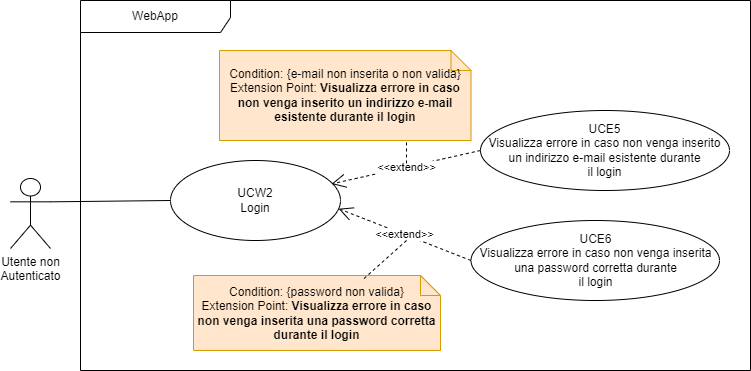
\includegraphics[scale=0.5]{UC_images/UCW2.png}
\caption{UCW2 - Login}
\end{figure}
\begin{itemize}
\item \textbf{Descrizione}: L'utente non autenticato accede alla piattaforma Sweeat.
\item \textbf{Attore primario}: Utente non autenticato.
\item \textbf{Precondizione}: L'utente non è ancora autenticato presso il sistema.
\item \textbf{Postcondizione}: L’utente ha effettuato l’accesso al sistema ed è all’interno del suo account.

\item \textbf{Scenario principale}:
\begin{enumerate}
\item L’utente accede al sistema;
\item L’utente seleziona la voce “Login”;
\item L’utente inserisce l’indirizzo e-mail con cui è registrato al sistema;
\item L’utente inserisce la password d’accesso; 
\item L’utente seleziona la voce “Accedi”. 
\end{enumerate}

\item \textbf{Estensioni}:
\begin{itemize}
\item Viene inserito un indirizzo e-mail errato 
\begin{enumerate}
	\item L’utente non può accedere al sistema;
	\item Viene mostrato un messaggio d’errore che indica che l'indirizzo e-mail inserito con cui accedere al sistema non è corretto (UCE5 §3.19). 
\end{enumerate}
\item Viene inserita una password errata
\begin{enumerate}
	\item L’utente non può accedere al sistema;
	\item Viene mostrato un messaggio d’errore che indica che la password inserita non è corretta (UCE6 §3.20).
\end{enumerate}
\end{itemize}
\end{itemize}